\section{Results and Discussion}
\label{sec:results}

\subsection{Experimental Setup and Quadruple-Precision Oracle}
To evaluate the numerical behavior of the proposed \texttt{Zvtakum} extension across scientific computing and machine learning workloads, we evaluate three benchmarks: (i) composite numerical quadrature rules (\texttt{make integracao}), (ii) Sparse Matrix-Vector Multiplication (SpMV) in Compressed Sparse Row (CSR) format, and (iii) a dense General Matrix-Vector Multiplication (GEMV) kernel. Unlike standard x86-64 \texttt{long double} (80-bit extended format with a 64-bit significand), our ground-truth reference $y_{\text{ref}}$ is computed in IEEE 754 quadruple precision (\texttt{\_\_float128} via \texttt{libquadmath}, providing 113 significand bits).

We compare linear Takum (\texttt{T8}, \texttt{T16}, \texttt{T32}) against IEEE 754~\cite{ieee754} \texttt{FP32} and \texttt{FP16}, as well as Open Compute Project (OCP) 8-bit formats~\cite{ocp_fp8} \texttt{OFP8 E4M3} (normal range up to $\pm 448$) and \texttt{OFP8 E5M2} (range up to $\pm 57344$). Two matrix dimensions are evaluated: $200 \times 200$ ($d = 10\%$, averaging 20 non-zeros per row) to exercise non-power-of-two strip-mining tails ($\texttt{vl} < \texttt{VLEN}/\texttt{SEW}$), and power-of-two dimensions ($256 \times 256$ SpMV with $d = 10\%, 20\%$ and $128 \times 128$ dense GEMV) that align evenly with a 128-bit vector register width ($\texttt{VLEN} = 128$, yielding $\texttt{vl} \in \{16, 8, 4\}$ elements per strip for \texttt{T8}, \texttt{T16}, and \texttt{T32}). To avoid division-by-near-zero distortion in element-wise relative error $\vert{}y_i - y_{\text{ref},i}\vert{} / \vert{}y_{\text{ref},i}\vert{}$, reference outputs satisfying $\vert{}y_{\text{ref},i}\vert{} \le 10^{-12} \max_j \vert{}y_{\text{ref},j}\vert{}$ are filtered out across 15 random seeds.

\subsection{Numerical Quadrature Validation}
Prior to vector workload evaluation, the arithmetic core was validated on composite numerical integration (trapezoidal quadrature of smooth transcendental integrands) across increasing subinterval counts $N$. Figure~\ref{fig:quadrature} illustrates the relative integration error as a function of discretization granularity. Both \texttt{T16} and \texttt{T32} closely track or surpass their IEEE counterparts before reaching rounding saturation, while \texttt{T8} remains bounded without catastrophic overflow as $N$ grows.

\begin{figure}[htbp]
\centering
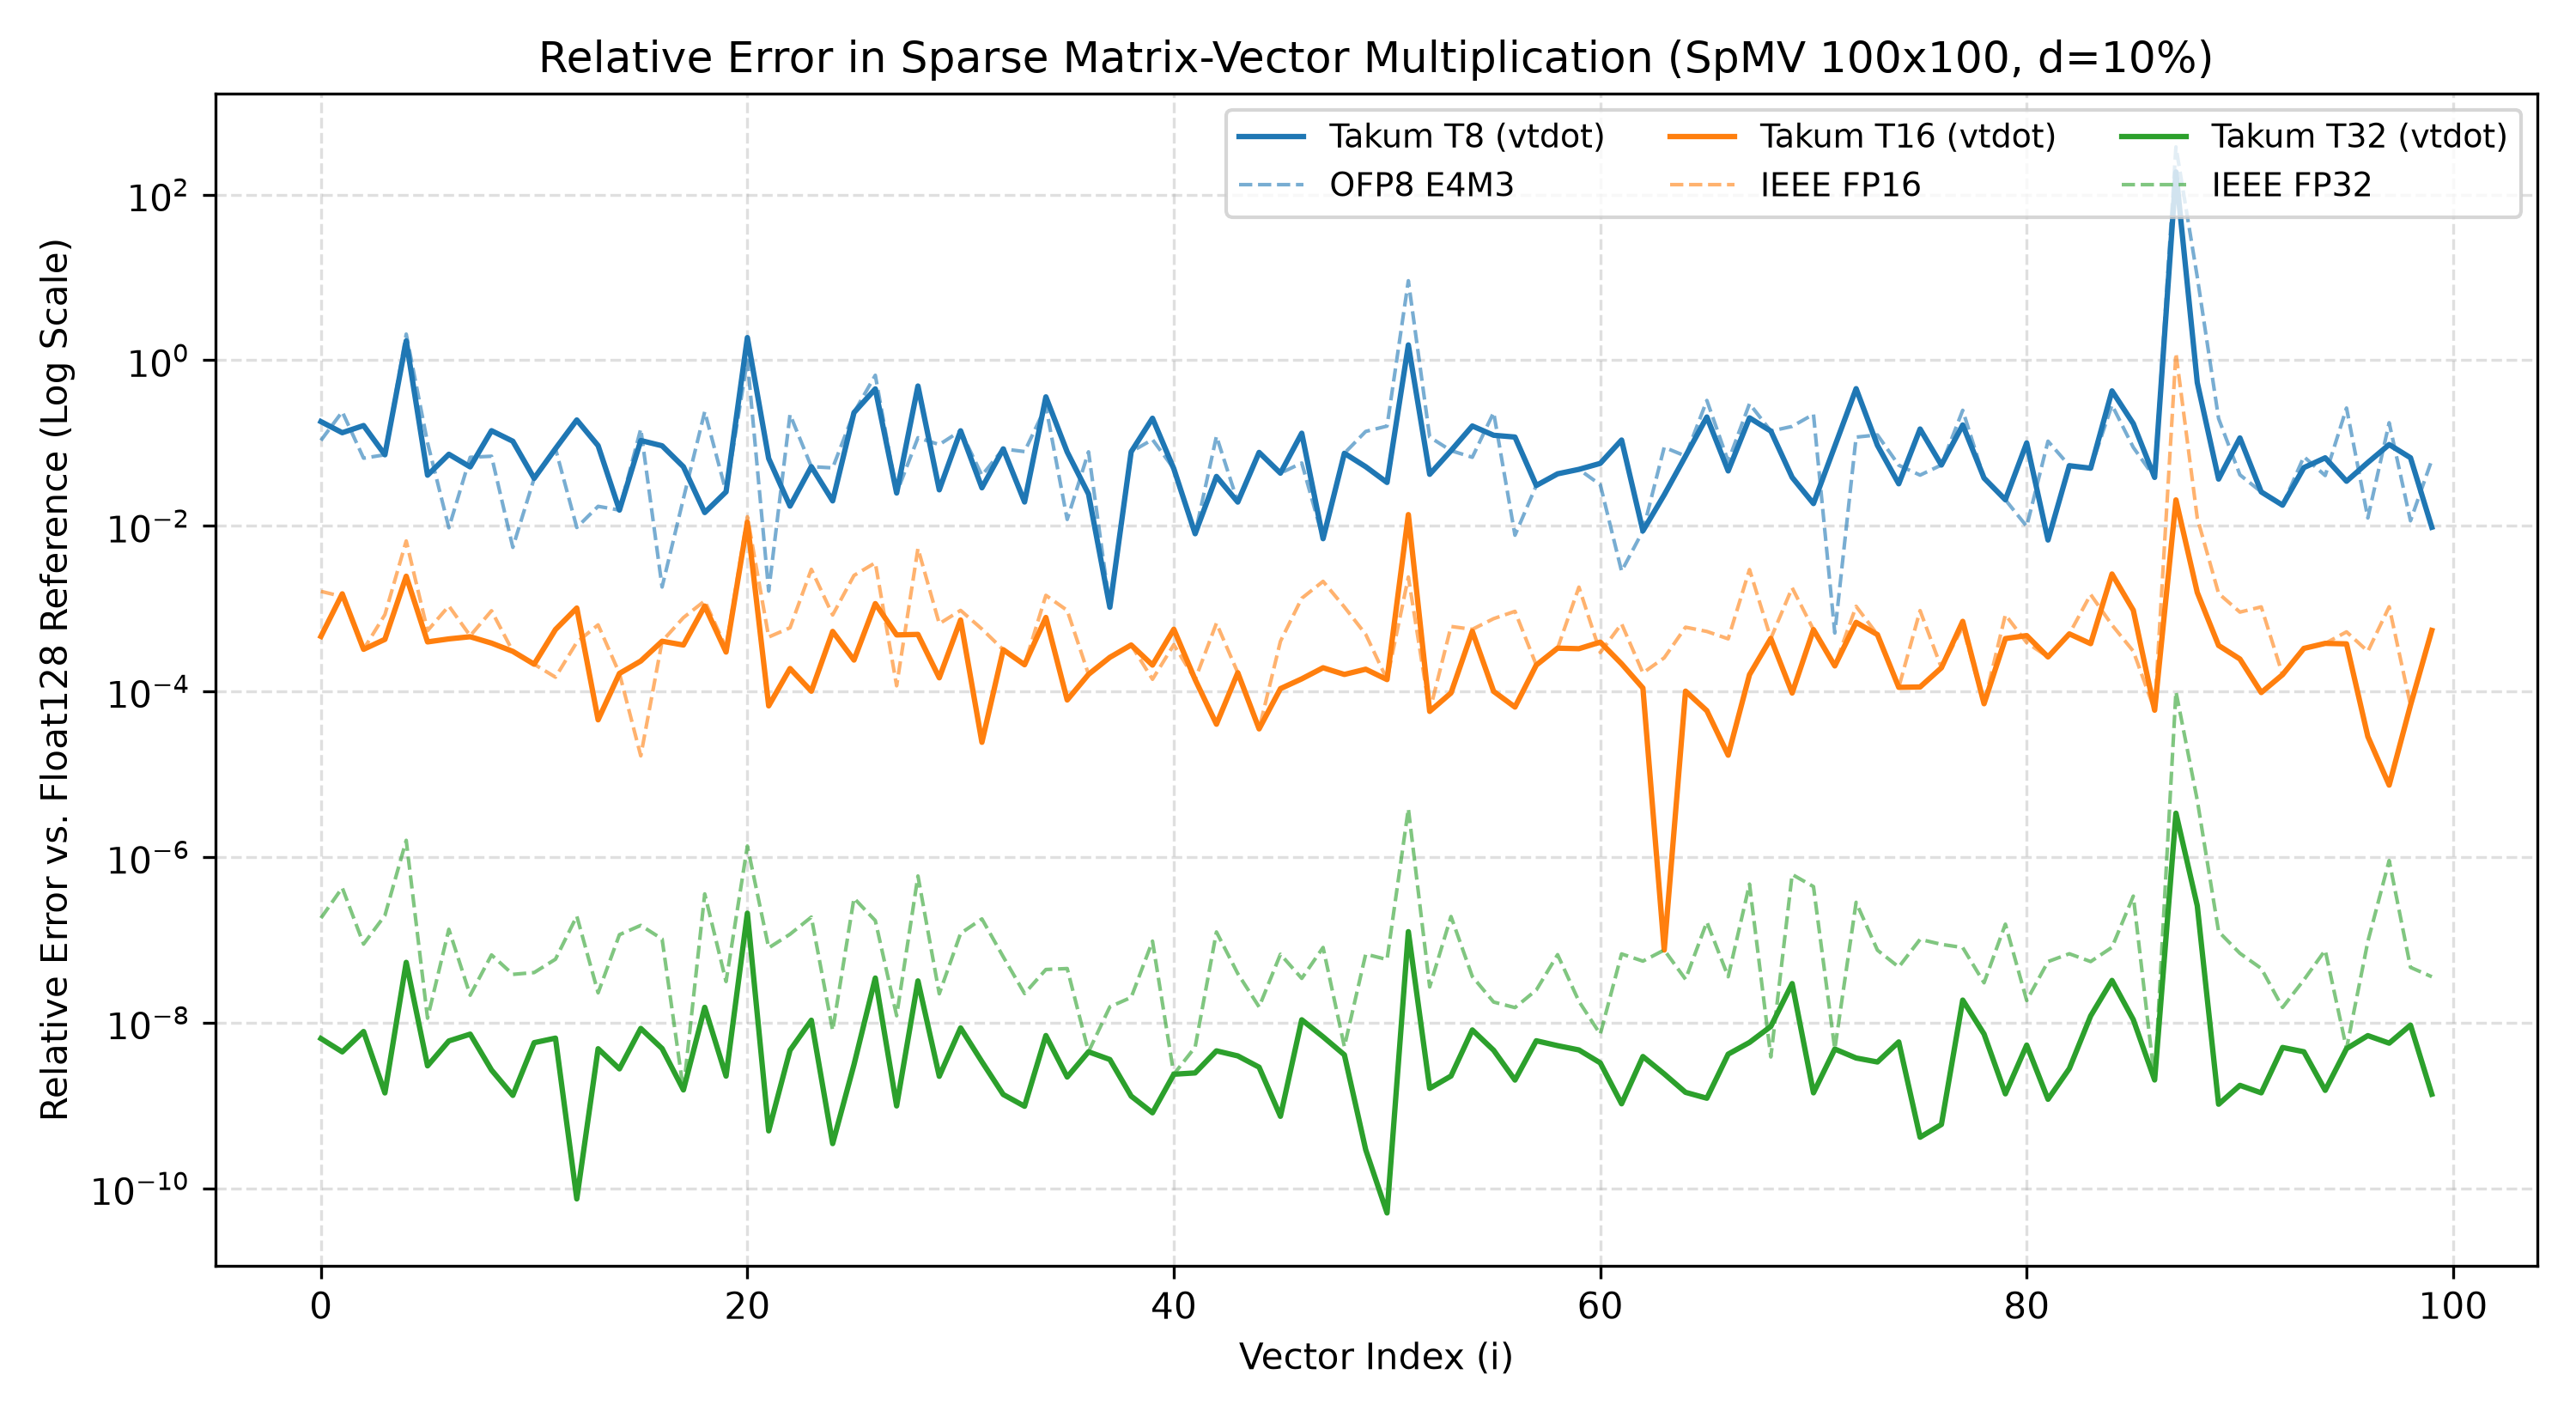
\includegraphics[width=0.95\columnwidth]{grafico_erro_takum.png}
\caption{Relative error in numerical quadrature validation across bitwidths.}
\label{fig:quadrature}
\end{figure}

\subsection{SpMV Accuracy: Narrow vs. Wide Dynamic Range}
Figure~\ref{fig:spmv_cdf} presents the Cumulative Distribution Function (CDF) of the element-wise relative error for $200 \times 200$ CSR sparse matrices ($d = 10\%$) under two input distributions: (a) a narrow standard normal regime $\mathcal{N}(0, 1)$, and (b) a wide dynamic range regime $\mathcal{N}(0, 1) \cdot 2^{\mathcal{U}(-18, 18)}$ whose products span roughly $2^{-36}$ to $2^{+36}$ ($\approx 10^{\pm 11}$).

\begin{figure*}[t]
\centering
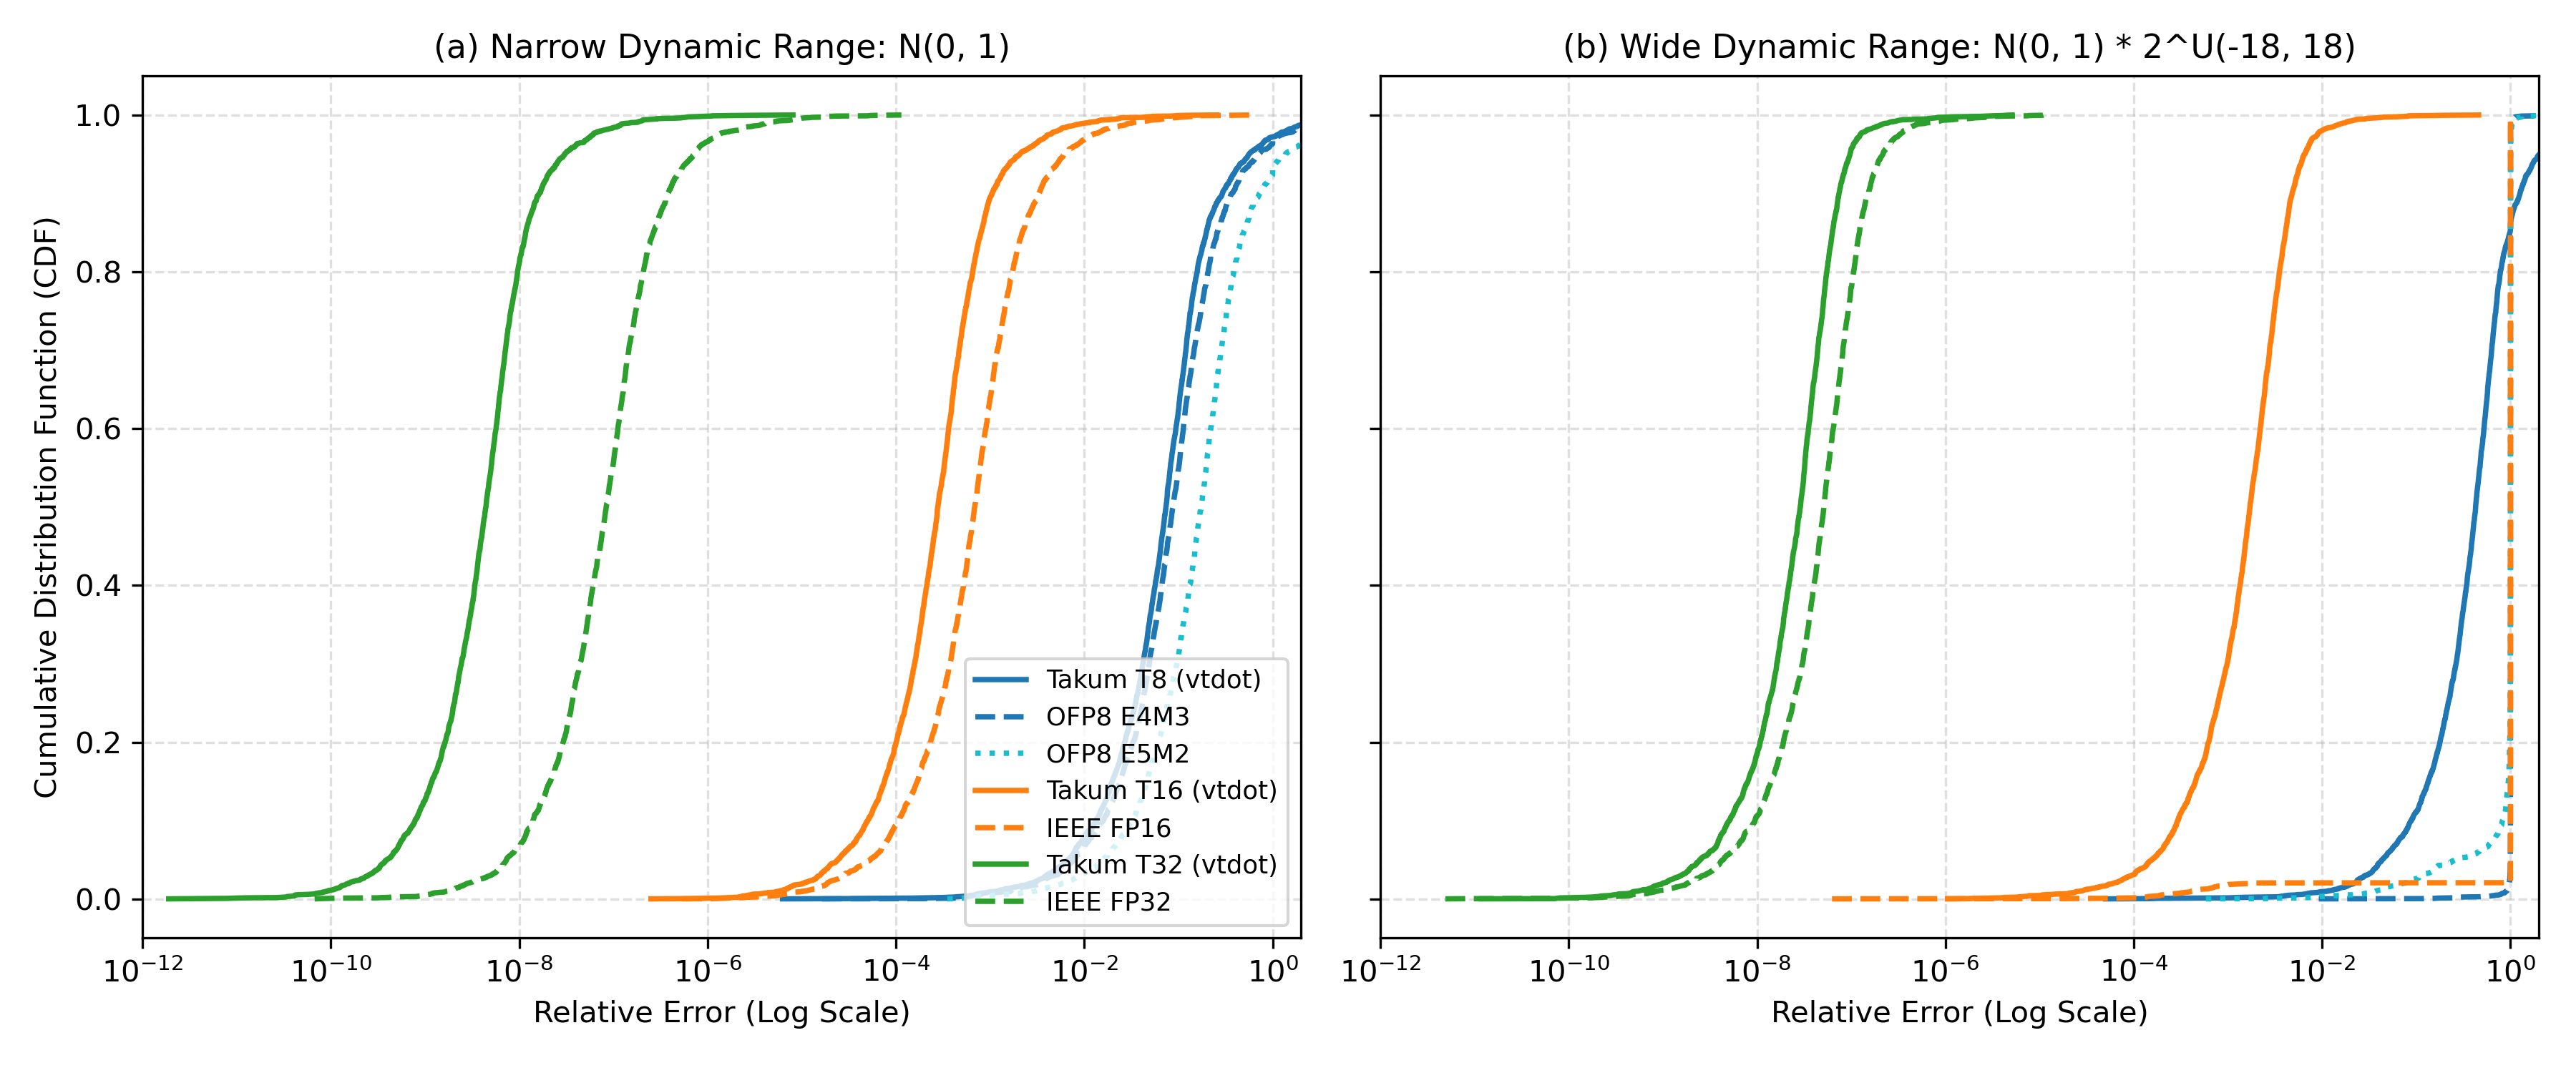
\includegraphics[width=0.92\textwidth]{grafico_cdf_spmv.png}
\caption{Cumulative Distribution Function (CDF) of element-wise relative error in CSR SpMV ($200 \times 200$, $d = 10\%$, 15 seeds) under (a) narrow $\mathcal{N}(0, 1)$ and (b) wide $\mathcal{N}(0, 1) \cdot 2^{\mathcal{U}(-18, 18)}$ dynamic range.}
\label{fig:spmv_cdf}
\end{figure*}

In the narrow regime (Fig.~\ref{fig:spmv_cdf}a), all formats operate within their normal exponent bounds. When paired with \texttt{vtdot.vv}, Takum achieves median relative errors of $7.44 \times 10^{-2}$ (\texttt{T8}), $2.63 \times 10^{-4}$ (\texttt{T16}), and $4.19 \times 10^{-9}$ (\texttt{T32}), improving upon chained \texttt{OFP8 E4M3} ($8.79 \times 10^{-2}$), \texttt{FP16} ($7.31 \times 10^{-4}$), and \texttt{FP32} ($8.68 \times 10^{-8}$).

In the wide dynamic range regime (Fig.~\ref{fig:spmv_cdf}b), the fixed exponent fields of \texttt{OFP8 E4M3}, \texttt{OFP8 E5M2}, and \texttt{FP16} suffer severe overflow and underflow, collapsing to a median relative error of $1.00 \times 10^{0}$ ($100\%$). Conversely, Takum completely avoids overflow and underflow across all bitwidths due to its tapered characteristic ($2^{\pm 255} \approx 10^{\pm 77}$ for \texttt{T16}/\texttt{T32} and $\approx 10^{\pm 72}$ for \texttt{T8}). While \texttt{T8} exhibits a high median relative error of $4.55 \times 10^{-1}$ ($45.5\%$) due to coarse 8-bit mantissa quantization at large exponents, it preserves order-of-magnitude information without saturating, whereas \texttt{T16} ($1.77 \times 10^{-3}$) and \texttt{T32} ($2.81 \times 10^{-8}$) maintain high accuracy.

\subsection{Disentangling Format Gain from Accumulator Gain}
To separate the intrinsic accuracy of the Takum format from the benefit of the wide internal accumulator in \texttt{vtdot.vv}, Figure~\ref{fig:dot_vs_chain} and Table~\ref{tab:gemv_spmv_breakdown} compare three accumulation modes:
\begin{enumerate}
    \item \textbf{Chained (\texttt{vtmul.vv} + \texttt{vtadd.vv}):} Element-wise multiplication followed by sequential addition rounded to \texttt{SEW} bits at every step (matching standard un-widened IEEE/OFP8 chaining);
    \item \textbf{Strip-Mined \texttt{vtdot.vv} ($\texttt{VLEN}=128$):} The hardware-realizable RVV execution mode where each strip of $\texttt{vl} = 128/\texttt{SEW}$ elements is accumulated in 64-bit internal precision and rounded back to \texttt{SEW} bits in \texttt{vd[0]} at the end of the strip;
    \item \textbf{Full-Row \texttt{vtdot.vv} (Full Acc):} An idealized upper bound where an entire row dot product is accumulated in 64-bit internal precision before a single final rounding to \texttt{SEW}. In hardware without a dedicated cross-strip accumulator CSR, this bound is only reached when the row non-zero count fits within a single vector strip ($nnz \le \texttt{VLEN}/\texttt{SEW}$).
\end{enumerate}

\begin{figure*}[t]
\centering
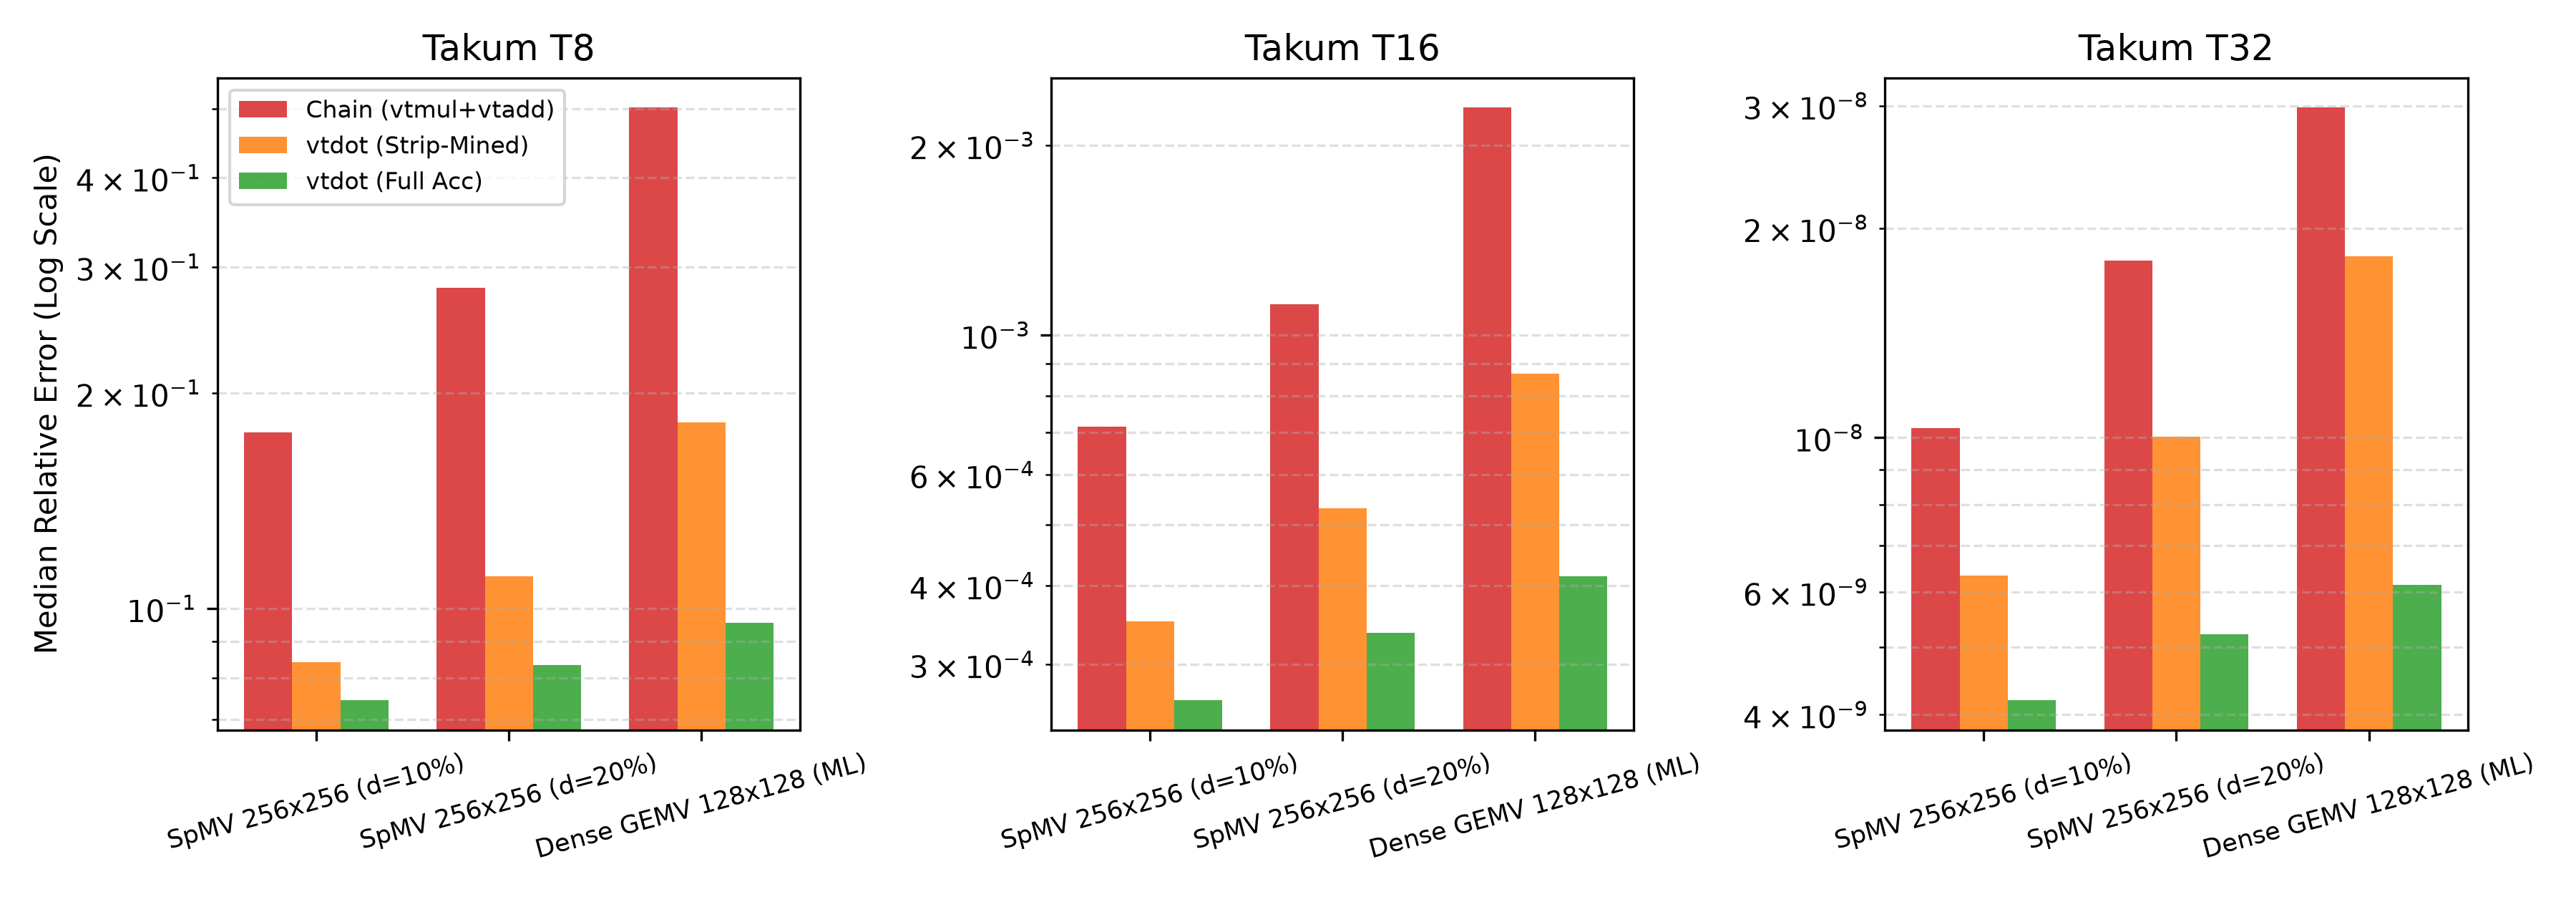
\includegraphics[width=0.92\textwidth]{grafico_dot_vs_chain.png}
\caption{Median relative error comparing chained accumulation (\texttt{vtmul.vv}+\texttt{vtadd.vv}), hardware strip-mined \texttt{vtdot.vv} ($\texttt{VLEN}=128$), and theoretical full-row \texttt{vtdot.vv} accumulation across SpMV ($256 \times 256$) and dense ML GEMV ($128 \times 128$).}
\label{fig:dot_vs_chain}
\end{figure*}

\begin{table}[htbp]
\centering
\caption{Median Relative Error Breakdown Across Accumulation Modes (Narrow Range $\mathcal{N}(0,1)$)}
\label{tab:gemv_spmv_breakdown}
\begin{tabular}{lccc}
\hline
\textbf{Format \& Mode} & \textbf{SpMV 10\%} & \textbf{SpMV 20\%} & \textbf{GEMV $128^2$} \\
\hline
\texttt{OFP8 E4M3} (Chained) & $1.02 \times 10^{-1}$ & $1.34 \times 10^{-1}$ & $1.81 \times 10^{-1}$ \\
\texttt{Takum T8} (Chained) & $1.78 \times 10^{-1}$ & $2.76 \times 10^{-1}$ & $4.92 \times 10^{-1}$ \\
\texttt{Takum T8} (\texttt{vtdot} Strip) & $8.12 \times 10^{-2}$ & $1.12 \times 10^{-1}$ & $1.76 \times 10^{-1}$ \\
\texttt{Takum T8} (\texttt{vtdot} Full) & $7.15 \times 10^{-2}$ & $8.04 \times 10^{-2}$ & $9.56 \times 10^{-2}$ \\
\hline
\texttt{IEEE FP16} (Chained) & $8.45 \times 10^{-4}$ & $1.15 \times 10^{-3}$ & $1.55 \times 10^{-3}$ \\
\texttt{Takum T16} (Chained) & $6.95 \times 10^{-4}$ & $1.10 \times 10^{-3}$ & $2.35 \times 10^{-3}$ \\
\texttt{Takum T16} (\texttt{vtdot} Strip) & $3.51 \times 10^{-4}$ & $5.32 \times 10^{-4}$ & $8.62 \times 10^{-4}$ \\
\texttt{Takum T16} (\texttt{vtdot} Full) & $2.68 \times 10^{-4}$ & $3.34 \times 10^{-4}$ & $4.14 \times 10^{-4}$ \\
\hline
\texttt{IEEE FP32} (Chained) & $9.80 \times 10^{-8}$ & $1.38 \times 10^{-7}$ & $1.87 \times 10^{-7}$ \\
\texttt{Takum T32} (Chained) & $1.03 \times 10^{-8}$ & $1.78 \times 10^{-8}$ & $2.98 \times 10^{-8}$ \\
\texttt{Takum T32} (\texttt{vtdot} Strip) & $6.25 \times 10^{-9}$ & $1.00 \times 10^{-8}$ & $1.82 \times 10^{-8}$ \\
\texttt{Takum T32} (\texttt{vtdot} Full) & $4.21 \times 10^{-9}$ & $5.28 \times 10^{-9}$ & $6.13 \times 10^{-9}$ \\
\hline
\end{tabular}
\end{table}

As shown in Table~\ref{tab:gemv_spmv_breakdown}, in narrow-range chained execution without a wide accumulator, \texttt{OFP8 E4M3} and \texttt{FP16} slightly outperform chained \texttt{T8} and \texttt{T16} on dense 128-element reductions because Takum devotes 5 header bits to $(S, D, R)$ to secure its wide dynamic range, leaving fewer mantissa bits at 8-bit width.

When using \texttt{vtdot.vv}, the $3\times$ to $7\times$ error reduction over chained Takum corresponds to the \textbf{Full-Row} accumulation bound ($9.56 \times 10^{-2}$ in \texttt{T8}, $4.14 \times 10^{-4}$ in \texttt{T16}, and $6.13 \times 10^{-9}$ in \texttt{T32}). Under realistic hardware \textbf{strip-mining ($\texttt{VLEN}=128$)}, each strip of $\texttt{vl}$ elements rounds its partial sum back to \texttt{SEW} bits in \texttt{vd[0]}. For \texttt{T16} ($\texttt{vl}=8$) and \texttt{T32} ($\texttt{vl}=4$), strip-mined \texttt{vtdot.vv} still reduces median error by $2.0\times$ to $2.7\times$ over chained Takum and outperforms chained \texttt{FP16} ($8.62 \times 10^{-4}$ vs. $1.55 \times 10^{-3}$) and \texttt{FP32} ($1.82 \times 10^{-8}$ vs. $1.87 \times 10^{-7}$). However, for \texttt{T8} on the dense $128 \times 128$ GEMV workload (8 strips of $\texttt{vl}=16$), the 8 intermediate roundings to 8-bit precision raise the strip-mined median error to $1.76 \times 10^{-1}$, making its accuracy comparable to chained \texttt{OFP8 E4M3} ($1.81 \times 10^{-1}$) when dynamic range is narrow, while retaining full immunity to overflow when inputs are unscaled.